\subsection{Residual correlations}
\label{sec:Residual}

In the hadronic rescattering phase of a heavy-ion collision, $\Lambda$ can scatter off of $\Sigma$, $\Xi$, and $\Omega$ baryons, though little is known about the cross section of these interactions.  
In principle, one could do a femtoscopic analysis of $\Lambda\Sigma^0$, $\Lambda\Xi^{-}$, or even $\Lambda\Omega$, in order to measure the scattering length and effective interaction range of these pairs. 
One could reconstruct many pairs of these particles, make correlation functions, and fit them with Eqn.\ \ref{eq:Lednicky}.
In practice, difficulties in topological reconstruction and small particle yields make such analyses challenging at best.
However, a ghost of these interactions haunts $\Lambda\Lambda$ femtoscopic analysis in the form of residual correlations.

The aforementioned hyperons all decay into $\Lambda$ baryons.  
The momentum difference between these particles and their daughter $\Lambda$ (caused by the decay) is small relative to the total momentum of the particles, such that daughter and parent carry very similar momenta.  
As a result, relative-momentum correlation functions between primary particles and secondary particles can be sensitive to the interactions between the primary particles and the parent particles.  
For example, the correlation between primary $\Lambda$ and primary $\Sigma^{\rm 0}$ should be visible, though somewhat smeared out, in the correlation between primary $\Lambda$ and secondary $\Lambda$.  
Furthermore, these secondary $\Lambda$ are often difficult to distinguish from primary $\Lambda$.  
Therefore, measurements of two-$\Lambda$ correlation functions will contain a mixture of primary correlations and feeddown correlations, and an attempt to parametrize the correlation functions should take this into account.  

In this analysis note, we will discuss two different methods of accounting for these residual correlations.  
In the "Transformed residuals method", the Lednicky equation is used to estimate the shape of the residual correlations \emph{before} they decay (e.g.\ to estimate the shape of the $\Lambda\Sigma$ correlation function in the $\Lambda\Sigma$ relative momentum space).  
This pre-feeddown correlation is then smeared into a residual correlation function (in the $\Lambda\Lambda$ momentum space) using a transform matrix that accounts for the kinematic effects of the decay of one or both of the particles.  
Different sources of residual correlations are determined separately and then summed together with the primary-primary correlation in the fit procedure.

In contrast, the "Gaussian residuals method" attempts to describe the full residual correlation effect phenomenologically.  
Rather than precisely describe each component of residual correlation, the full shape of the residual correlation is described with a Gaussian parametrization.  


\subsubsection{Transformed residuals method}
\label{sec:TransformedResiduals}


One example of the transformed residuals method can be seen in the recent analysis \cite{Kisiel:2014mma} of STAR p$\bar{\Lambda}$ correlation functions measured in 200 GeV Au--Au collisions.  
In this study, p$\bar{\Lambda}$ and $\bar{\mathrm{p}}\Lambda$ correlations were fit with and without residual correlations.  
The fits with residual correlations included feeddown and feedup contributions from numerous sources.  
The study found that the fit with residual correlations measured a source size comparable to the previously measured sizes of p$\Lambda$ and $\bar{\mathrm{p}}\bar{\Lambda}$.  
In contrast, the fits that did not include residual correlations measured source radii that deviated significantly from the old p$\Lambda$ and $\bar{\mathrm{p}}\bar{\Lambda}$ results.  
One conclusion from that study was that it is important to make a precise characterization of the $\lambda$ parameters associated with each type of pair contribution.  
As mentioned above in Section \ref{sec:Observables}, the $\lambda$ parameter can be interpreted as the fraction of total pairs associated with that pair type.  
Quantitatively, it is included in the fit as shown in Equation \ref{eq:Residual} below.

We attempt to quantify the residual contamination in this analysis by simultaneously fitting the data for both the primary correlation function and the residual correlations.  
For example, $\Lambda\Lambda$ correlations with $\mathrm{\Lambda\Sigma^0}$ feeddown would be fit using 

\begin{equation}
\label{eq:Residual}
C_{\mathrm{meas}}(k^*_{\Lambda\Lambda})= 1 + \lambda_{\Lambda\Lambda}[C_{\Lambda\Lambda}(k^*_{\Lambda\Lambda})-1]+\lambda_{\Lambda\Sigma}[C_{\Lambda\Sigma}(k^*_{\Lambda\Lambda})-1],
\end{equation}
where 
\begin{equation}
\label{eq:ResCorSmear}
C_{\Lambda\Sigma}(k^*_{\Lambda\Lambda}) \equiv \frac{\displaystyle\sum\limits_{k^*_{\Lambda\Sigma}}T(k^*_{\Lambda\Lambda},k^*_{\Lambda\Sigma})C_{\Lambda\Sigma}(k^*_{\Lambda\Sigma})}{\displaystyle\sum\limits_{k^*_{\Lambda\Sigma}}T(k^*_{\Lambda\Lambda},k^*_{\Lambda\Sigma})},
\end{equation}
$C_{\Lambda\Sigma}(k^*_{\Lambda\Sigma})$ is the $\Lambda\Sigma$ correlation function calculated from Eq.~(\ref{eq:Lednicky}), and $T$ is a transform matrix generated with THERMINATOR \cite{Chojnacki:2011hb}, which shows how the $k^*$ of pairs of particles kinematically transforms when one of the particles decays.  
Figure \ref{fig:TherminatorLS} shows the normalized transform matrix for $\Lambda\Sigma \rightarrow \Lambda\Lambda$.
The width of the smearing band is characterized by the decay momentum --- 74 MeV/c for $\Sigma^0 \rightarrow \Lambda + \gamma$.
See Section \ref{sec:SmearMath} for details about the normalization.


\begin{figure}[hbtp]
\begin{center}
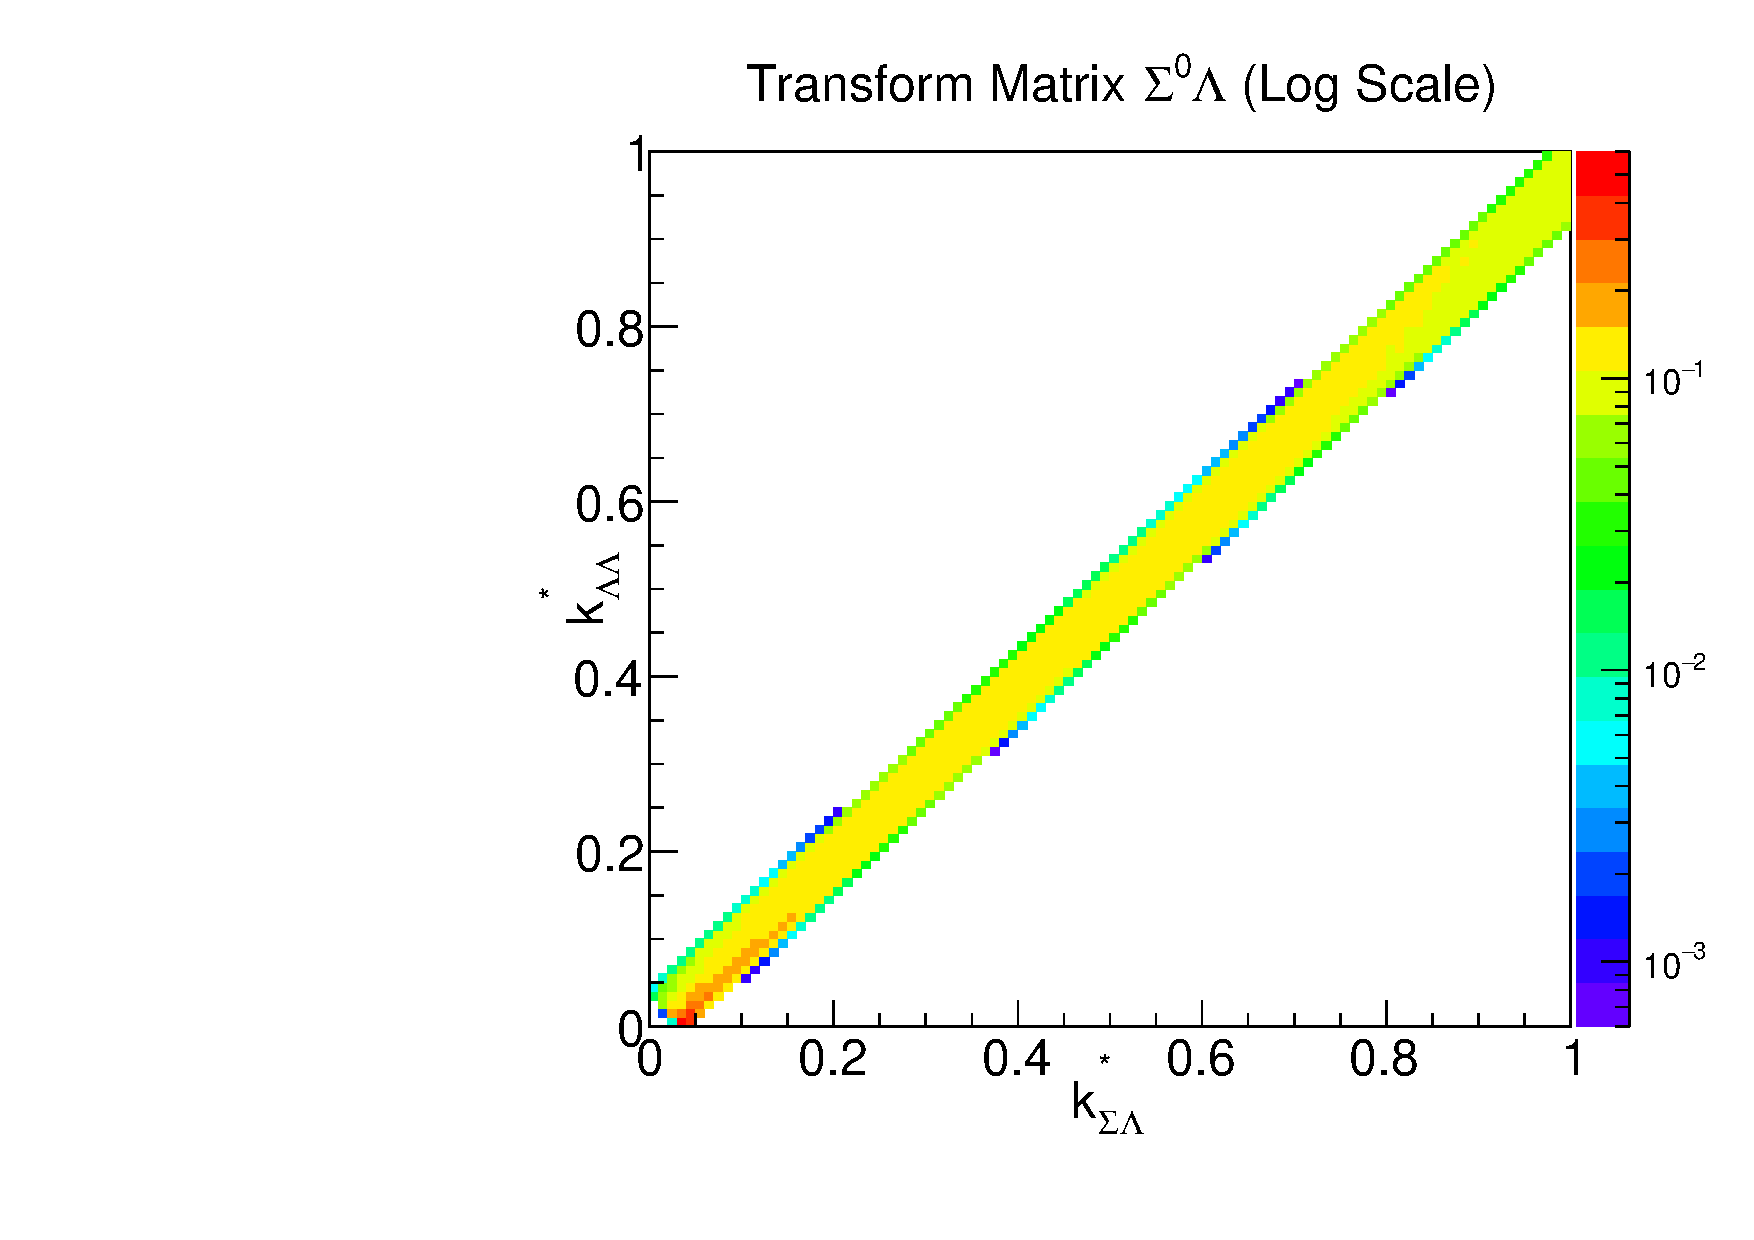
\includegraphics[width=24pc]{Figures/TransformMatrices/2016-7-20-TransformMatrixSigmaLambdaNormLog.pdf}
\end{center}
\caption[Transform matrix for $k^*_{\Sigma^0\Lambda} \rightarrow k^*_{\Lambda\Lambda}$]{THERMINATOR \cite{Chojnacki:2011hb} transform matrix showing how the relative momentum of $\Sigma^0\Lambda$ pairs transforms into relative momentum of $\Lambda\Lambda$ pairs after the $\Sigma^0$ decays. Each row is normalized to unity.}
\label{fig:TherminatorLS}
\end{figure}

Further residual correlations (e.g.\ from $\Sigma\Sigma \rightarrow \Lambda\Lambda$) can be included via additional terms.
The generalized form of Eqn.\ \ref{eq:Residual} is 
\begin{equation}
\label{eq:GeneralizedLambda}
C_{\mathrm{meas}}(k^*_{\Lambda\Lambda})= \sum_{i} \lambda_{i} C_{i}(k^*_{\Lambda\Lambda}),
\end{equation}
where $i$ runs over the different pair types, and $\sum \lambda_{i} = 1$.
Figures \ref{fig:TherminatorSS}--\ref{fig:TherminatorXcX0} show normalized residual correlations for $\Sigma^0\Lambda$, $\Sigma^0\Sigma^0$, $\Sigma^0\Xi^{0}$, $\Sigma^0\Xi^{-}$, $\Xi^0\Lambda$ $\Xi^{-}\Lambda$, and $\Xi^0\Xi^{-}$. 
The width of double hyperon decays $YY \rightarrow \Lambda\Lambda$ is generally wider than single decays $Y\Lambda \rightarrow \Lambda\Lambda$ because each decay contibrutes a momentum shift.
The antihyperon decays $\bar{Y} \rightarrow \bar{\Lambda}$ have the same kinematics as the hyperon decays, so Figures \ref{fig:TherminatorLS}--\ref{fig:TherminatorXcX0} are also used for their respective antiparticle-antiparticle and particle-antiparticle pair smearing.

\begin{figure}[hbtp]
\begin{center}
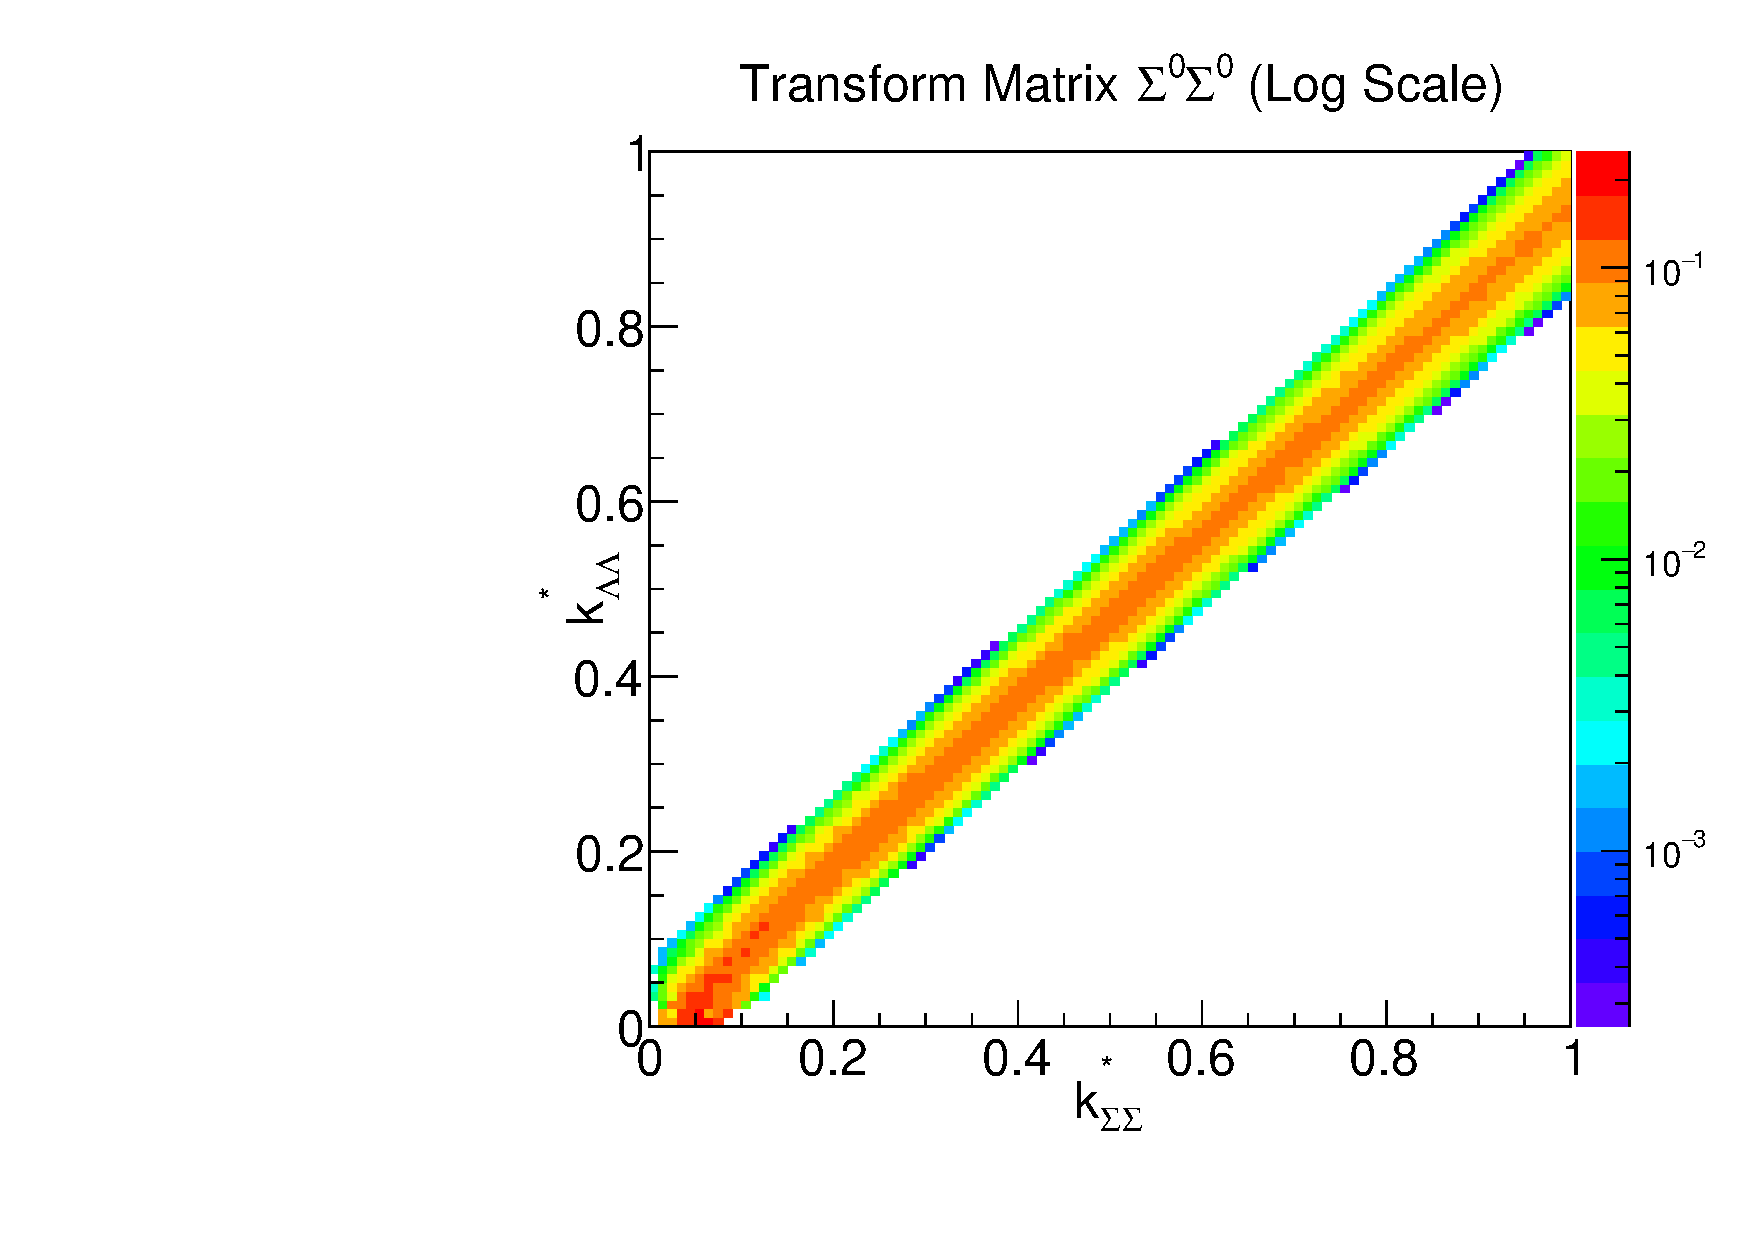
\includegraphics[width=24pc]{Figures/TransformMatrices/2016-7-20-TransformMatrixSigmaSigmaNormLog.pdf}
\end{center}
\caption[Transform matrix for $k^*_{\Sigma^0\Sigma^0} \rightarrow k^*_{\Lambda\Lambda}$]{THERMINATOR \cite{Chojnacki:2011hb} transform matrix showing how the relative momentum of $\Sigma^0\Sigma^0$ pairs transforms into relative momentum of $\Lambda\Lambda$ pairs after both $\Sigma^0$ have decayed. Each row is normalized to unity. The smearing effect is wider here than for $\Sigma^0\Lambda$ because there are two decays happening.}
\label{fig:TherminatorSS}
\end{figure}

\begin{figure}[hbtp]
\begin{center}
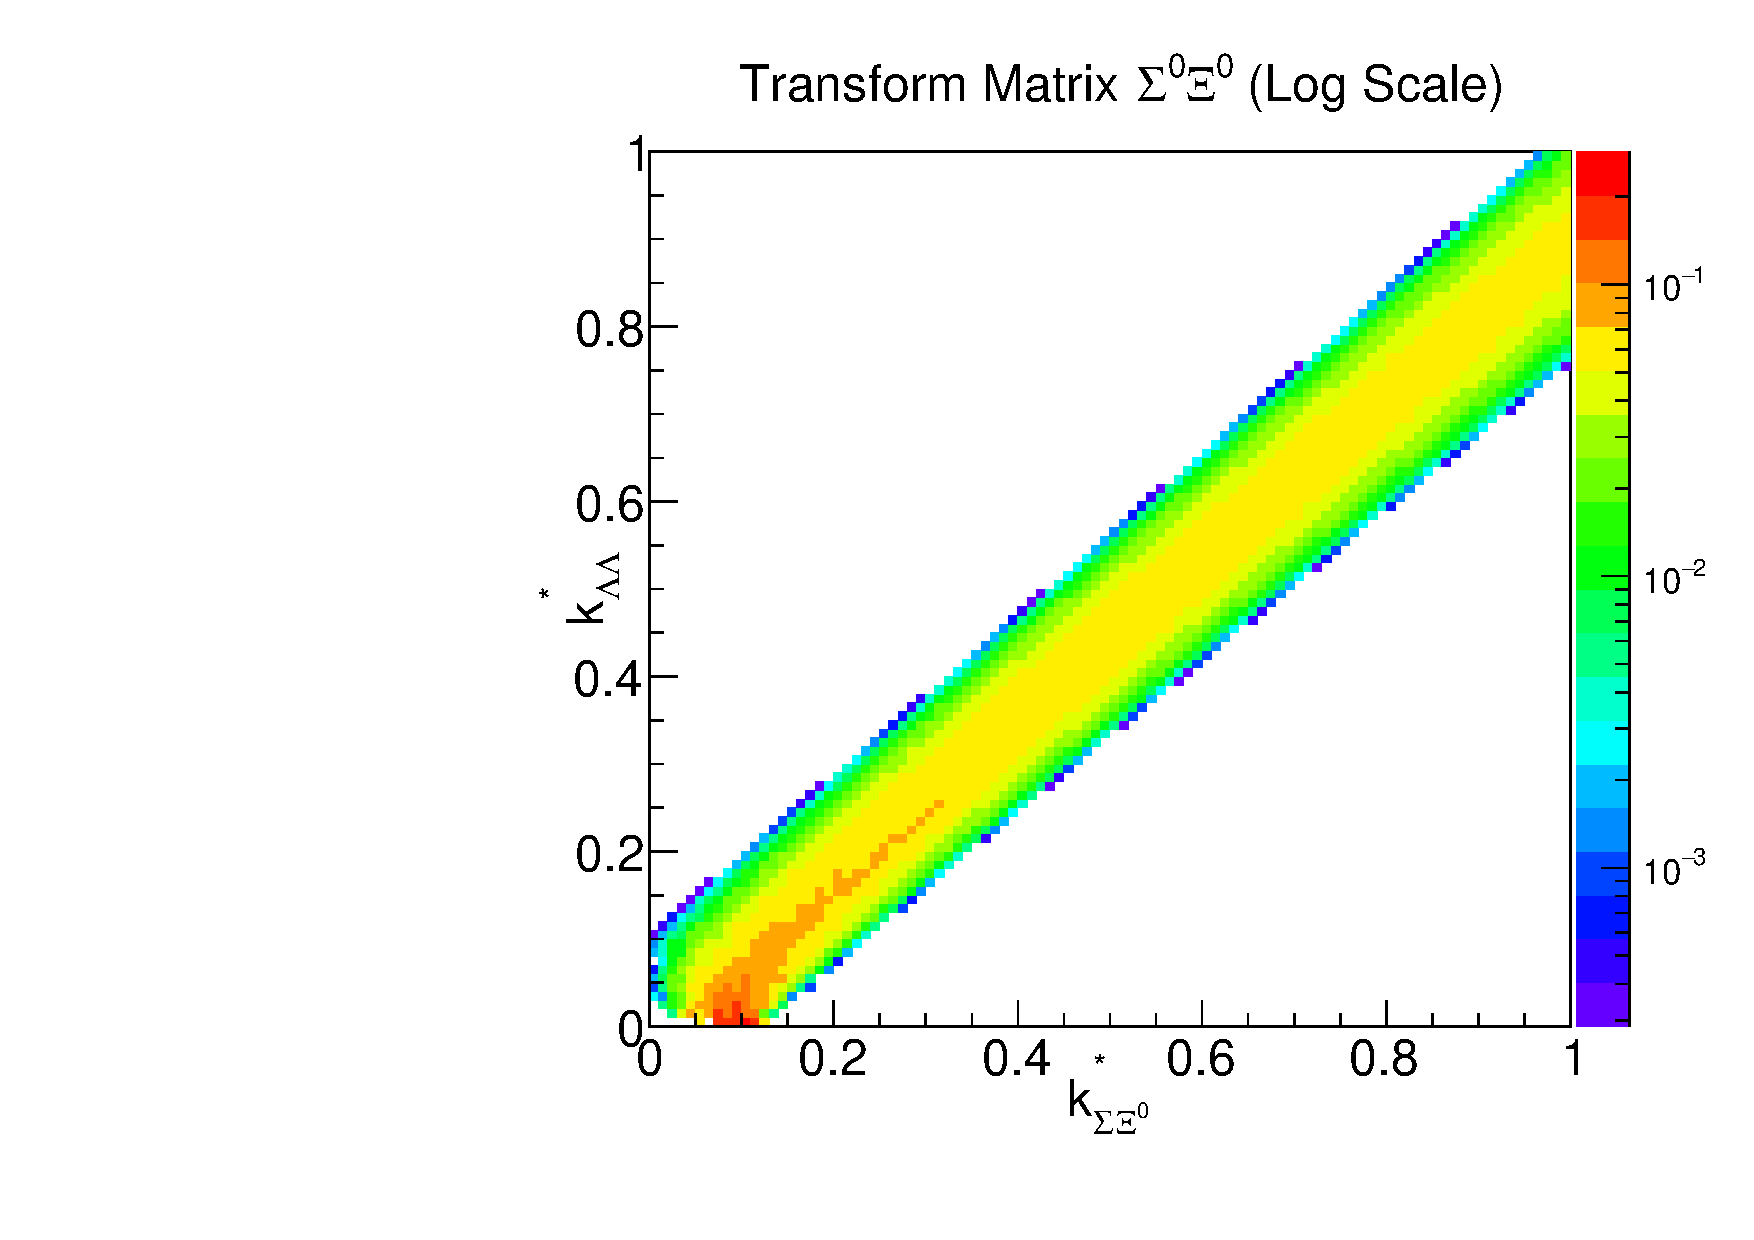
\includegraphics[width=24pc]{Figures/TransformMatrices/2016-7-20-TransformMatrixSigmaXi0NormLog.pdf}
\end{center}
\caption[Transform matrix for $k^*_{\Sigma^0\Xi^0} \rightarrow k^*_{\Lambda\Lambda}$]{THERMINATOR \cite{Chojnacki:2011hb} transform matrix showing how the relative momentum of $\Sigma^0\Xi^0$ pairs transforms into relative momentum of $\Lambda\Lambda$ pairs after both parents have decayed. Each row is normalized to unity. The smearing effect is wider here than for $\Sigma^0\Lambda$ because there are two decays happening.}
\label{fig:TherminatorSX0}
\end{figure}

\begin{figure}[hbtp]
\begin{center}
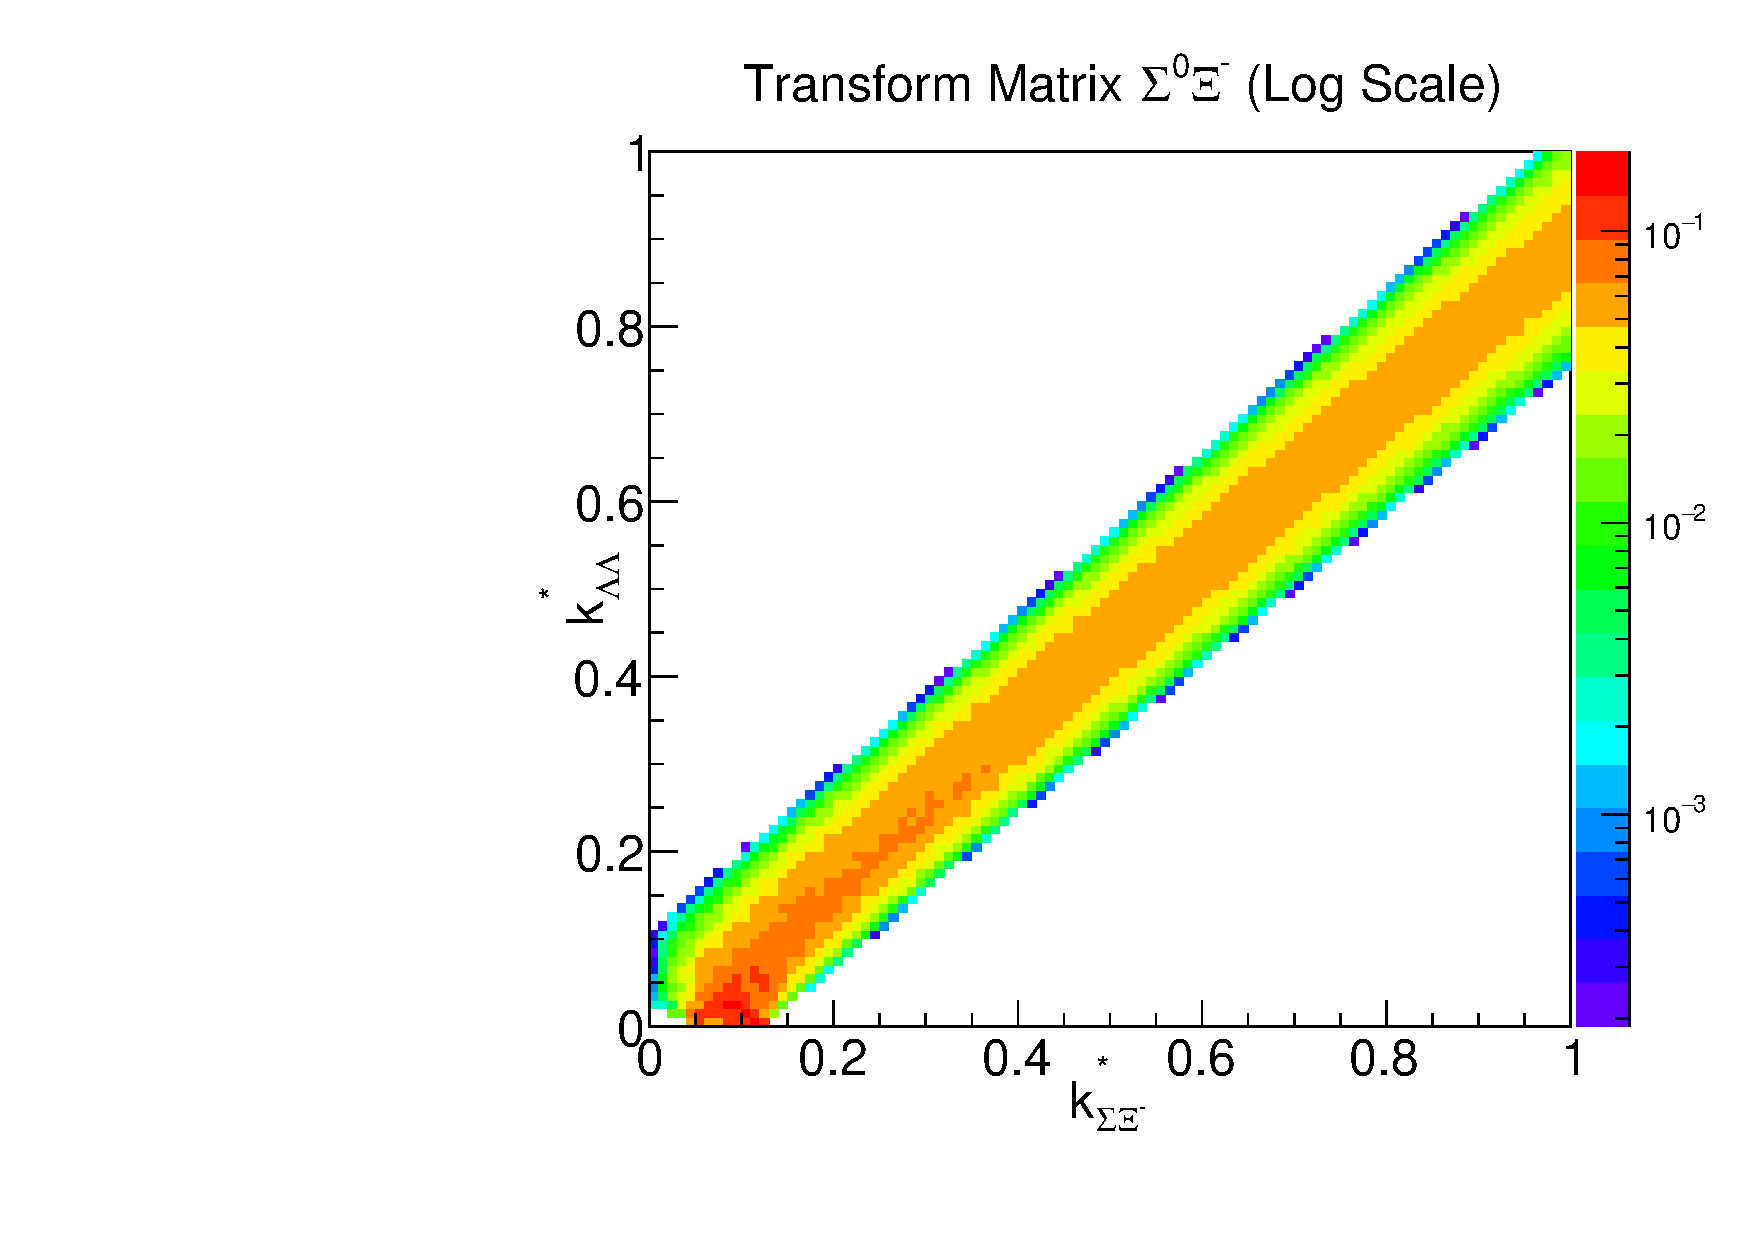
\includegraphics[width=24pc]{Figures/TransformMatrices/2016-7-20-TransformMatrixSigmaXiCNormLog.pdf}
\end{center}
\caption[Transform matrix for $k^*_{\Sigma^0\Xi^-} \rightarrow k^*_{\Lambda\Lambda}$]{THERMINATOR \cite{Chojnacki:2011hb} transform matrix showing how the relative momentum of $\Sigma^0\Xi^-$ pairs transforms into relative momentum of $\Lambda\Lambda$ pairs after both parents have decayed. Each row is normalized to unity. The smearing effect is wider here than for $\Sigma^0\Lambda$ because there are two decays happening.}
\label{fig:TherminatorSXc}
\end{figure}

\begin{figure}[hbtp]
\begin{center}
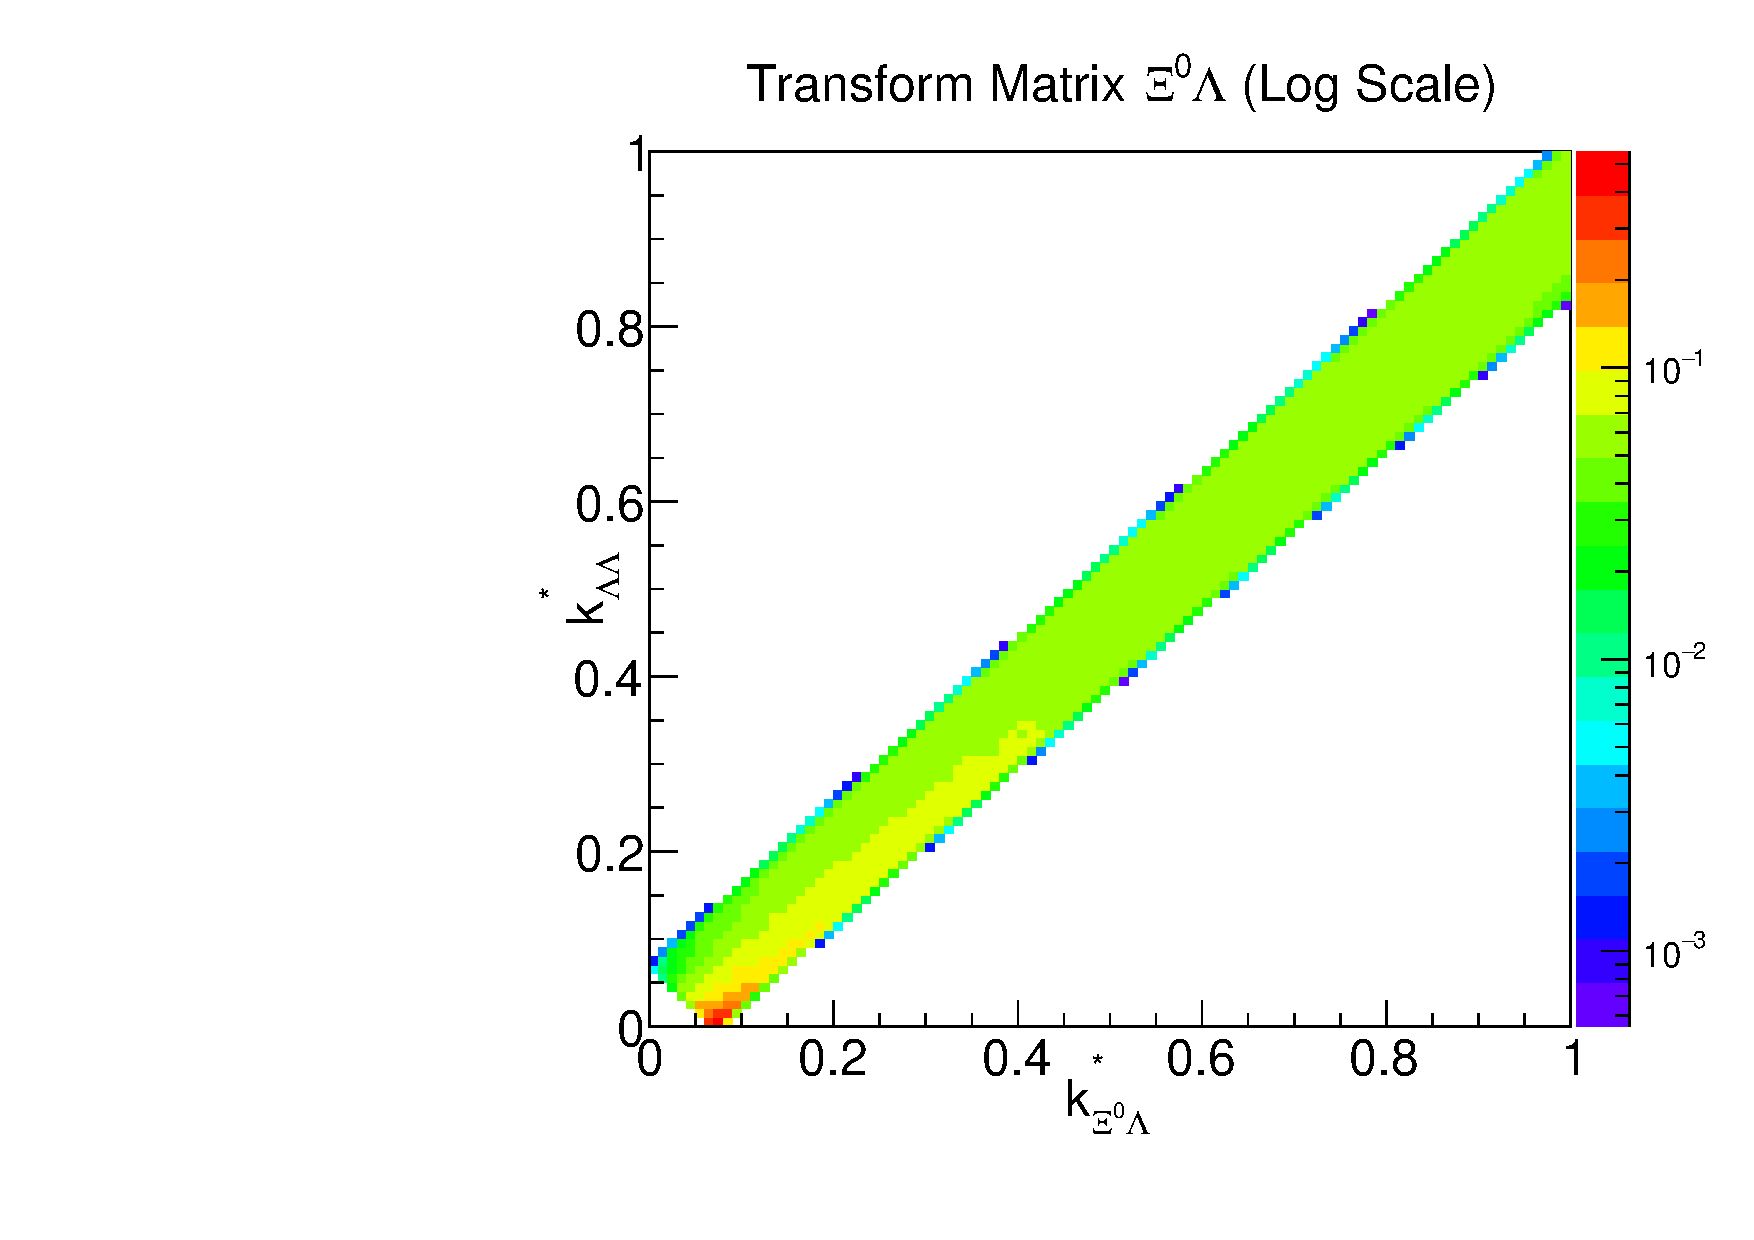
\includegraphics[width=24pc]{Figures/TransformMatrices/2016-7-20-TransformMatrixXi0LambdaNormLog.pdf}
\end{center}
\caption[Transform matrix for $k^*_{\Xi^0\Lambda} \rightarrow k^*_{\Lambda\Lambda}$]{THERMINATOR \cite{Chojnacki:2011hb} transform matrix showing how the relative momentum of $\Xi^0\Lambda$ pairs transforms into relative momentum of $\Lambda\Lambda$ pairs after the $\Xi^0$ has decayed. Each row is normalized to unity.}
\label{fig:TherminatorX0L}
\end{figure}

\begin{figure}[hbtp]
\begin{center}
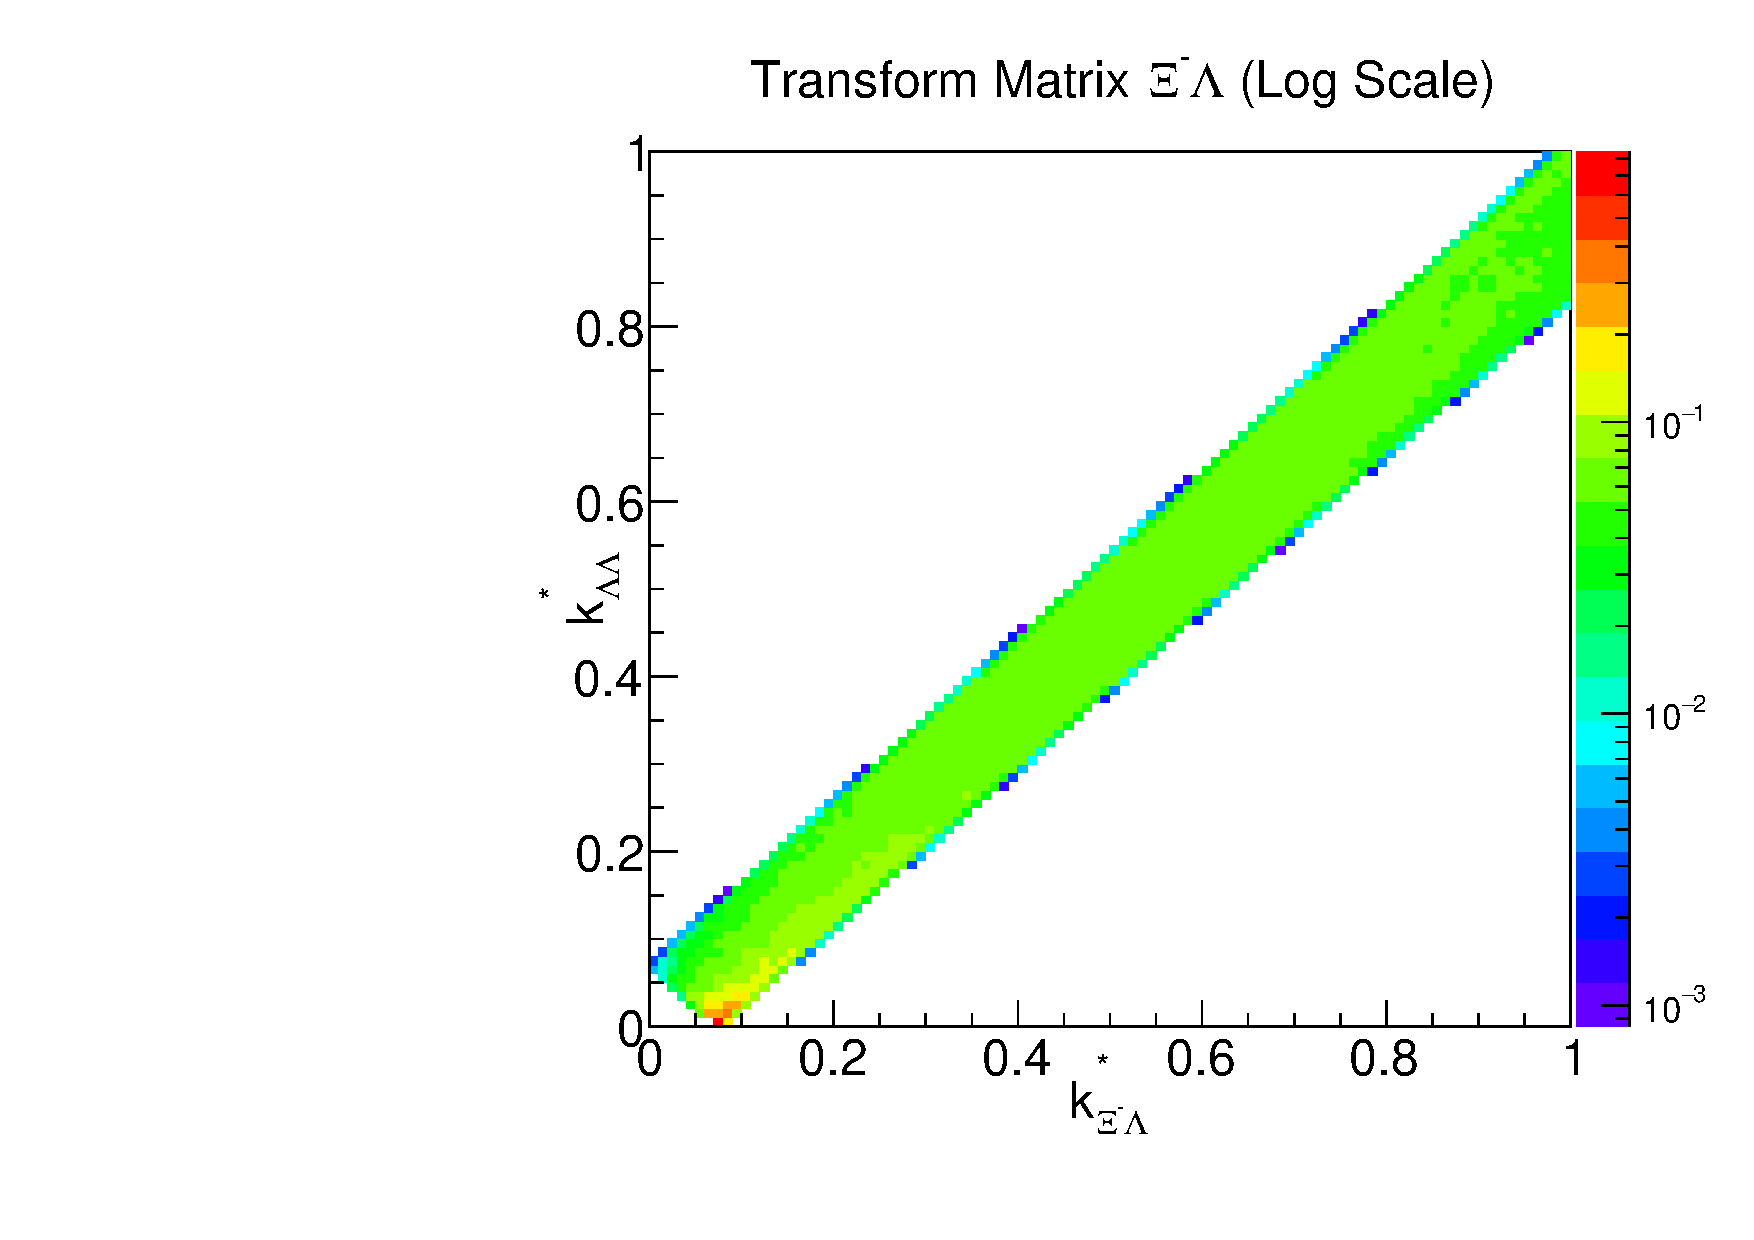
\includegraphics[width=24pc]{Figures/TransformMatrices/2016-7-20-TransformMatrixXiCLambdaNormLog.pdf}
\end{center}
\caption[Transform matrix for $k^*_{\Xi^-\Lambda} \rightarrow k^*_{\Lambda\Lambda}$]{THERMINATOR \cite{Chojnacki:2011hb} transform matrix showing how the relative momentum of $\Xi^-\Lambda$ pairs transforms into relative momentum of $\Lambda\Lambda$ pairs after the $\Xi^-$ has decayed. Each row is normalized to unity.}
\label{fig:TherminatorXcL}
\end{figure}

\begin{figure}[hbtp]
\begin{center}
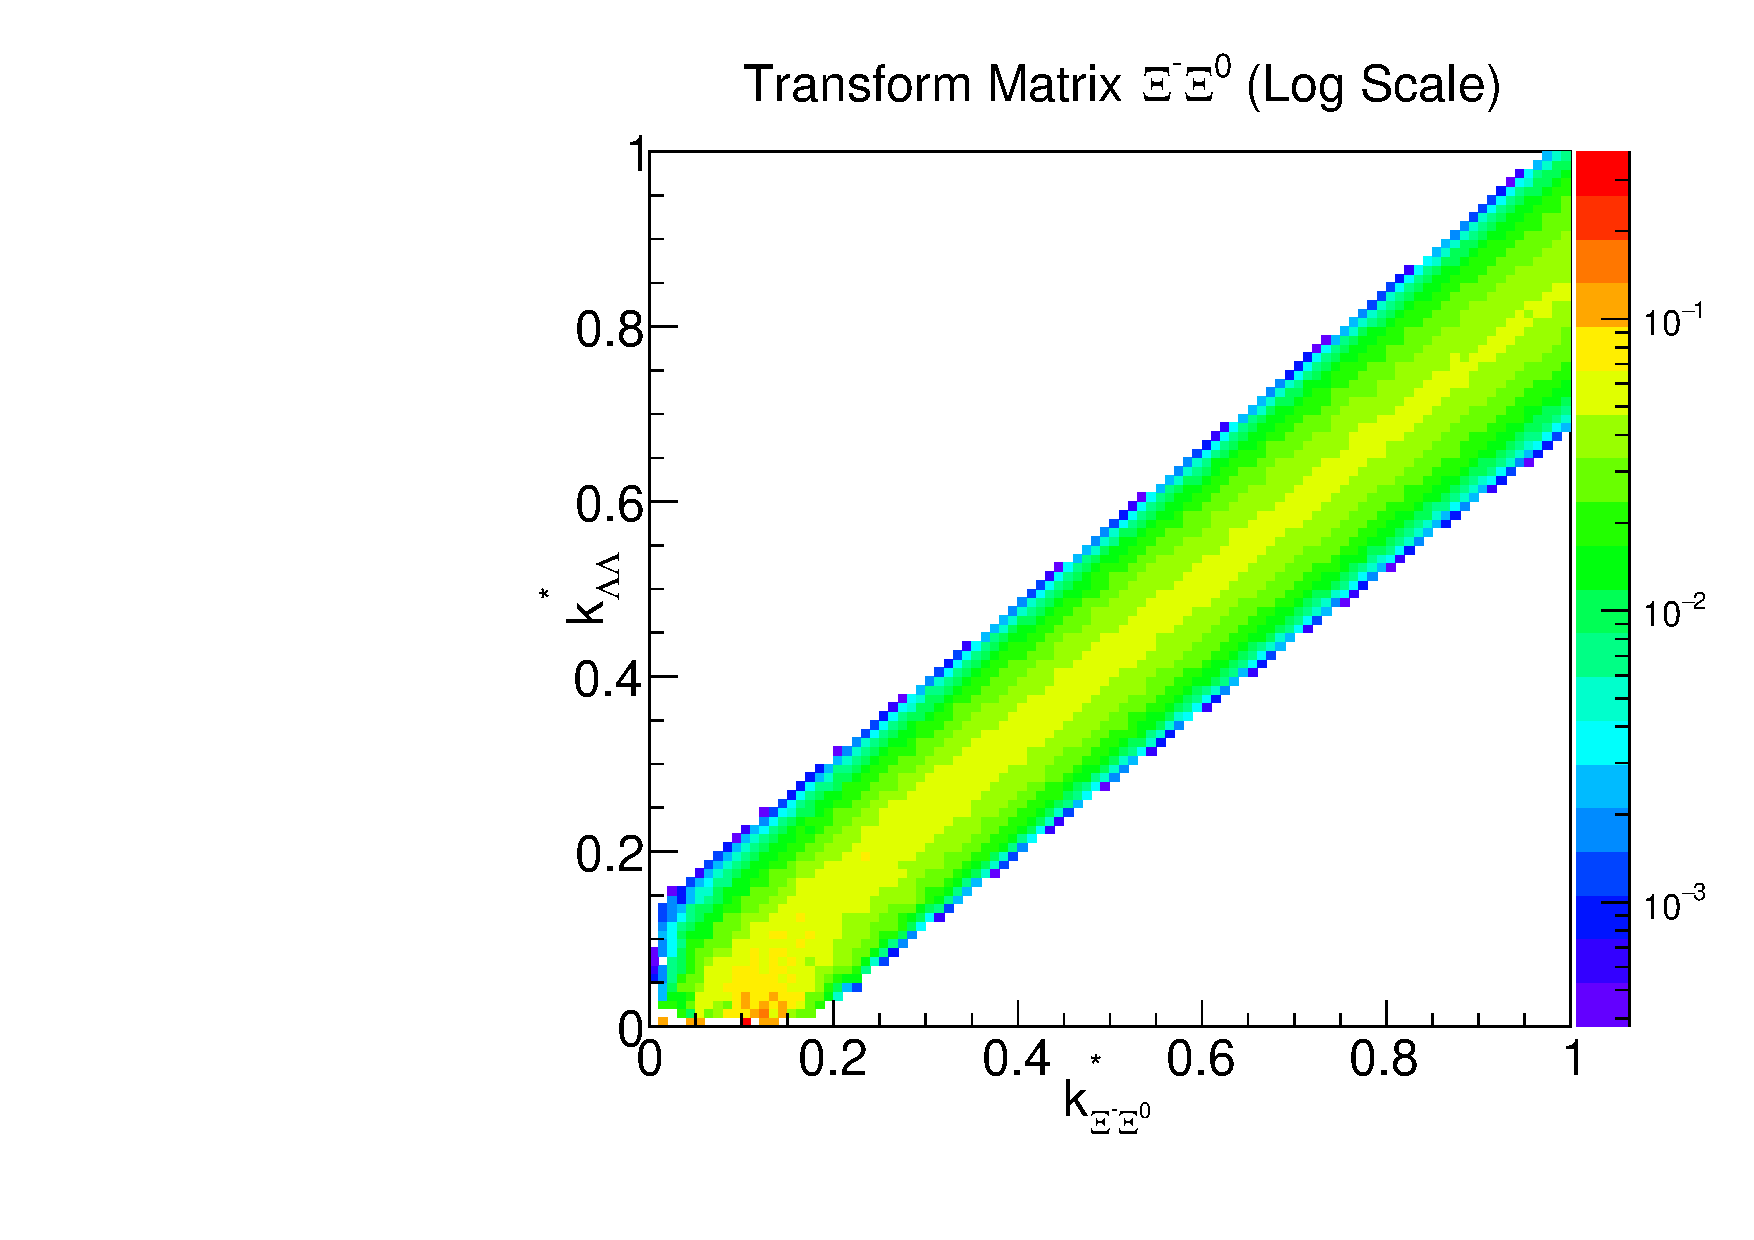
\includegraphics[width=24pc]{Figures/TransformMatrices/2016-7-20-TransformMatrixXiCXi0NormLog.pdf}
\end{center}
\caption[Transform matrix for $k^*_{\Xi^-\Xi^0} \rightarrow k^*_{\Lambda\Lambda}$]{THERMINATOR \cite{Chojnacki:2011hb} transform matrix showing how the relative momentum of $\Xi^-\Xi^0$ pairs transforms into relative momentum of $\Lambda\Lambda$ pairs after the both parents have decayed. Each row is normalized to unity. The smearing effect is wider here than for $\Sigma^0\Lambda$ because there are two decays happening.}
\label{fig:TherminatorXcX0}
\end{figure}

In a simple case with only two pair types ($\Lambda\Lambda$ and $\Lambda\Sigma$), the $\lambda$ parameters could either be fixed to some estimated experimental value, or they could be left as free fit parameters.
However, in this analysis it is necessary to account for all the pair types discussed above.
See Section \ref{sec:LambdaParamEstimates} for estimates of $\lambda$ parameters as well as estimates of which residual correlations must be included and which can be safely neglected.  
Because each residual correlation is calculated using the Lednicky equation, it is necessary to estimate, fit, or otherwise constrain the femtoscopic radius, $R$, and scattering parameters, $f_0$ and $d_0$, of the residual correlation pair.
Those constraints are described further in Section \ref{sec:ScatteringParams}.

\subsubsection{Gaussian residuals method}
\label{sec:GaussianResiduals}

The Gaussian residuals method has been used  to fit the STAR p$\bar{\Lambda}$ data \cite{Shapoval:2014yha}, as well as 200 GeV STAR $\Lambda\Lambda$ data \cite{Adamczyk:2014vca}.

In the Gaussian residual method, the measured correlation function is fit with 

\begin{equation}
\label{eq:GaussianResiduals}
C_{\mathrm{meas}}(k^*) = \lambda_{\mathrm{prim}}*C_{\mathrm{prim}}(k^*)+(1-\lambda_{\mathrm{prim}})(1-\beta  e^{-4k^{*2}\omega^2})
\end{equation}

where the phenomenological parameters $\beta$ and $\omega$ help fit the roughly Gaussian-shaped residual correlations that are expected.
The interpretation of $\beta$ and $\omega$ is tenuous, so if one has reasonable estimates for the different components ($\lambda$ parameters) of the residual correlations, as well as for the strength of the residual interactions (the scattering parameters $f_0$ and $d_0$), one is probably better off using the more rigorous Transform method of Section \ref{sec:TransformedResiduals}.
%advantages: Don't need to know/make big assumptions about residual interaction parameters.

%disadvantages:  Hard to interpret fit parameters.  Might conflict 




